Visualization of the systems was implemented in the form of a webpage. The webpage is served via frontend service and once fetched it keeps communicating with the backend service in order to serve the most recent information about the system. As service is exposed through ingress resources it is available externally from any machine connected to the internet. A real, working website example can be seen in the Figure \ref{fig:frontend}.

The user journey begins by selecting the system from the "Systems" dropdown menu. This menu is filled  while fetching the webpage. After selecting the system, its state will be shown in the main area of the webpage. The state will be visualized as a grid map with agents' positions marked as colored dots and starting and goal positions as colored squares. In cases where the path is not yet planned, agents won't be shown on the map. On the right side of the main area, a list of the agents along with the machine's name will be displayed, crown symbolize that this particular agent is a leader.

\begin{figure}[H]
    \centering
    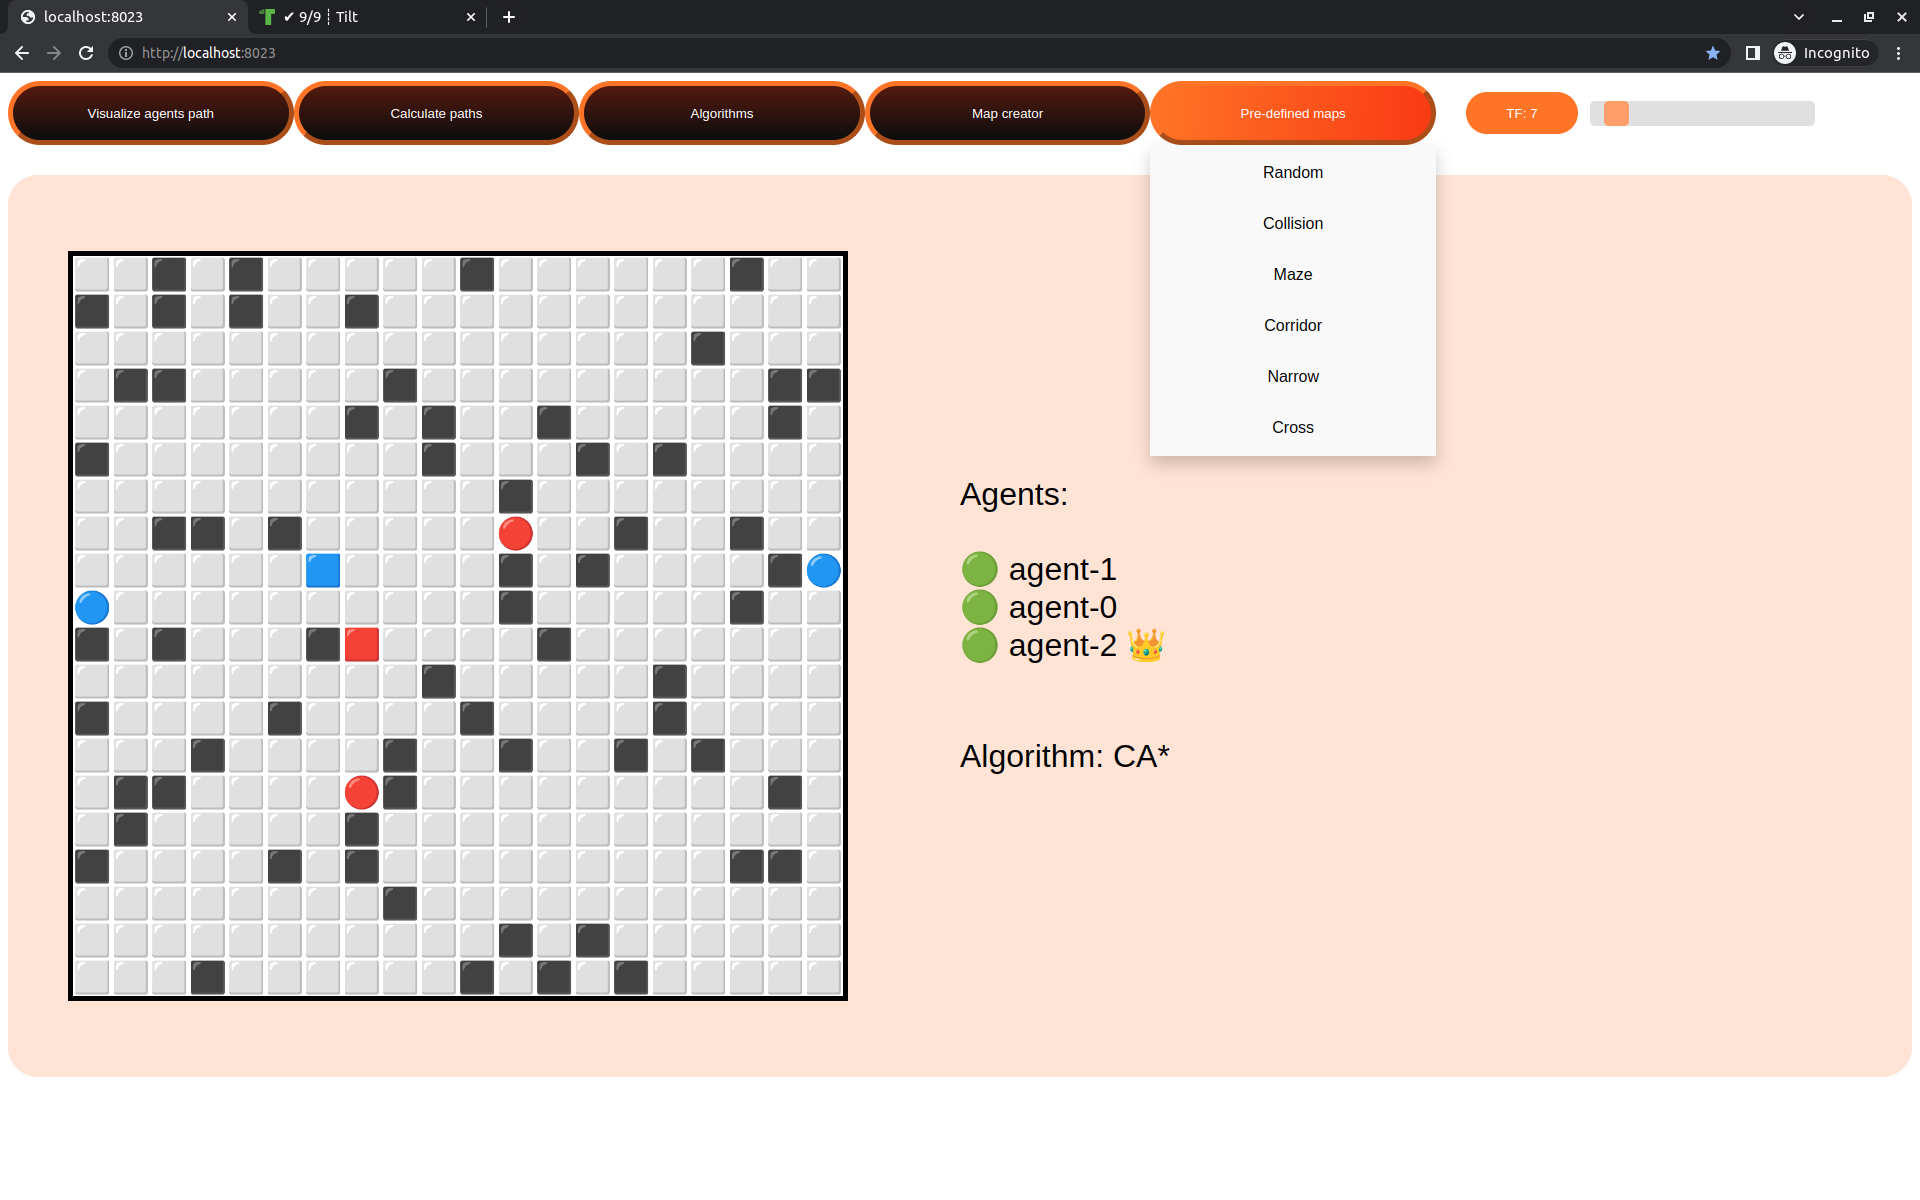
\includegraphics[width=\textwidth]{pictures/frontend.png}
    \caption{Frontend website} 
    \label{fig:frontend}
\end{figure}

Users can interact with a webpage by selecting a predefined map for the agents, and selecting an algorithm that should be used for calculation. After calculating the path, it can be visualized as an animation or replayed step by step using the slider located in the top right of the web page.

Additionally, the user can create his own map by accessing "map-creator". Once selected user will be asked about the size of the map and shown a map of that size meant for marking the walls and agents' position. An example of a "map-creator" view can be seen in the Figure \ref{fig:map-creator}.

\begin{figure}[H]
    \centering
    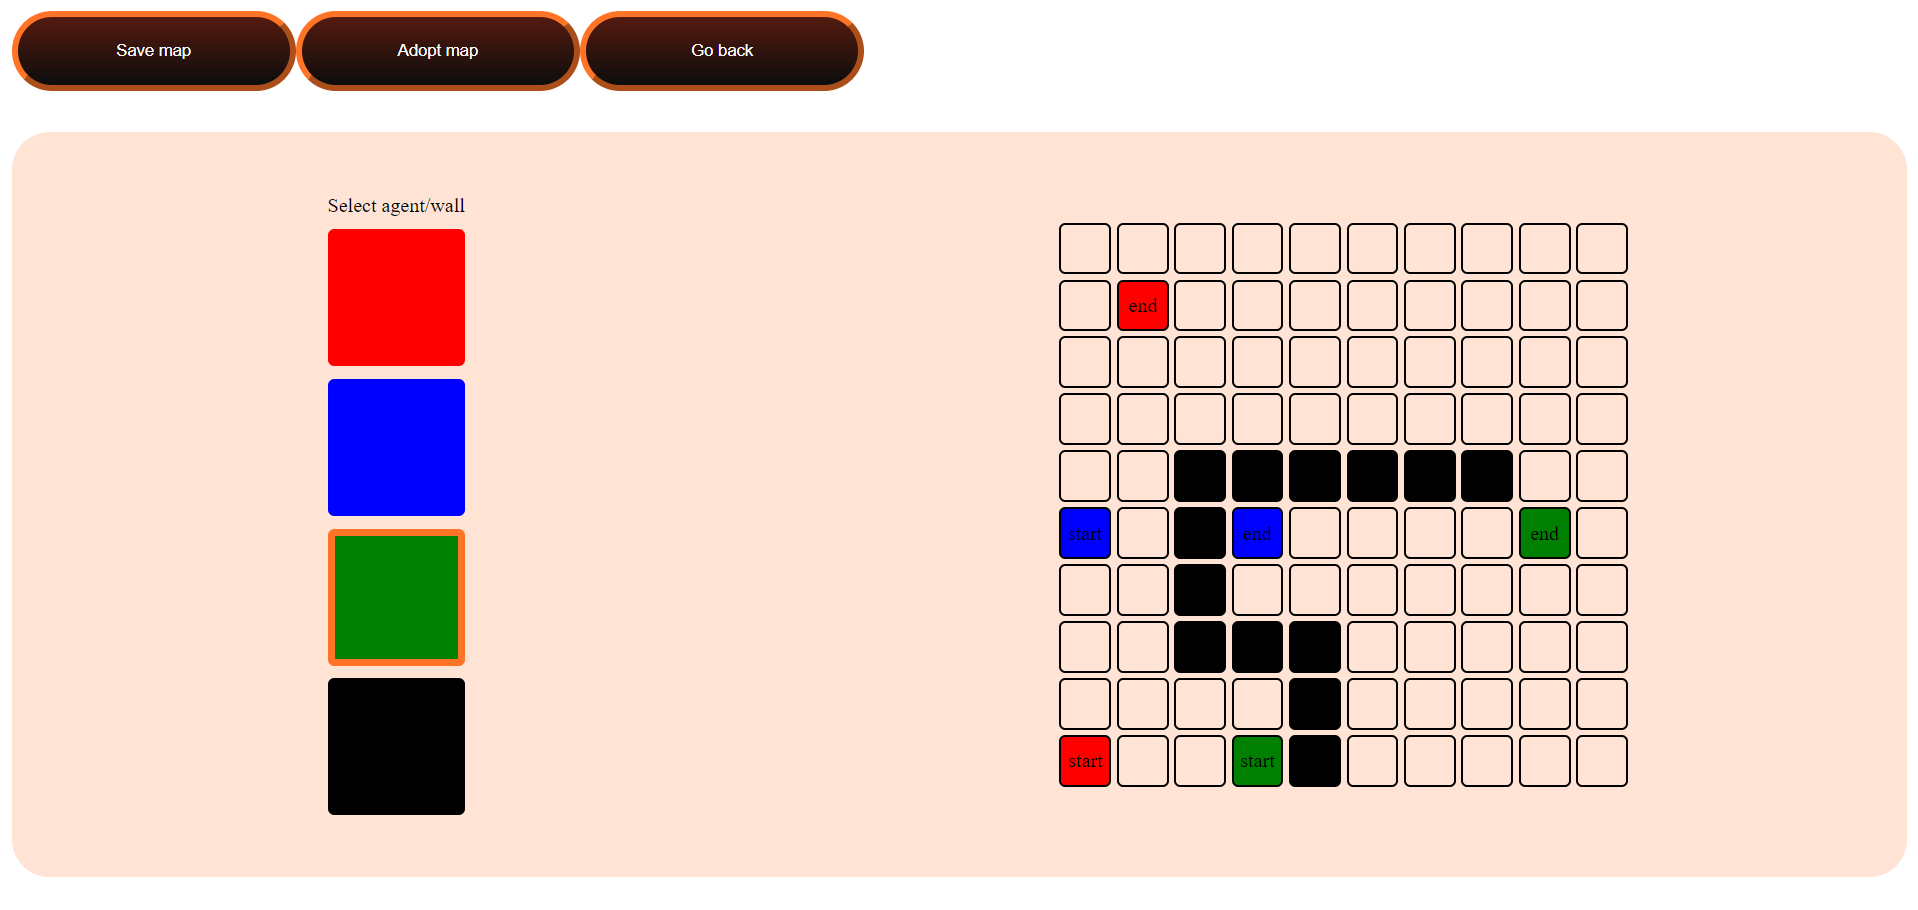
\includegraphics[width=0.8\textwidth]{pictures/map-creator.png}
    \caption{Frontend map-creator} 
    \label{fig:map-creator}
\end{figure}